% Fachvortrag - Evolutionsstrategien - Jannis Weber + Niklas Hartinger - Praktikum Künstliche Intelligenz
\documentclass[%
	BCOR=8.25mm,         % Bindekorrektur
	DIV=12,              % Satzspiegel
	parskip=half,				 % Abstand zwischen Absätzen
	bibliography=totoc,	 % Literaturverzeichnis im Inhaltsverzeichnis
	headsepline=on,      % Trennlinie Kolumnentitel
	cleardoublepage=plain % page numbers on standard cleared double pages
	]{scrartcl}

%% Präambel
\usepackage[english, ngerman]{babel} % deutsche typogr. Regeln + Trenntabelle
\usepackage[T1]{fontenc}             % interner TeX-Font-Codierung
\usepackage{lmodern}                 % Font Latin Modern
\usepackage[utf8]{inputenc}          % Font-Codierung der Eingabedatei
\usepackage[babel]{csquotes}         % Anführungszeichen
\usepackage{graphicx}                % Graphiken
\usepackage{booktabs}                % Tabellen schöner
\usepackage{listingsutf8}            % Listings mit Einstellungen
\lstset{basicstyle=\small\ttfamily,
	tabsize=2,
	basewidth={0.5em,0.45em},
	extendedchars=true}
\usepackage{amsmath}	               % Mathematik
\usepackage[pdftex]{hyperref}
\hypersetup{
	bookmarksopen=true,
	bookmarksopenlevel=3,
	colorlinks=true,
	citecolor=black,
	linkcolor=black,
	urlcolor=magenta
}
\usepackage{scrhack}								 % unterdrückt Fehlermeldung von listings

%% Verzeichnisse
\usepackage{tocstyle} 
\usetocstyle{KOMAlike}

%% Nummerierungstiefen
\setcounter{tocdepth}{3}             % 3 Stufen im Inhaltsverzeichnis
\setcounter{secnumdepth}{3} 		     % 3 Stufen in Abschnittnummerierung




% CUSTOM ADDED PACKAGES START HERE

\usepackage{float}
\usepackage{caption}
\usepackage{subcaption}
%\usepackage[automake, acronym]{glossaries}
\usepackage{tabulary}
\usepackage{tikz}
\usepackage{listings}
\usepackage{color}
\usepackage{pdflscape}
\usepackage{tocloft}
\usepackage{amssymb}
\usepackage{xurl}

\usepackage[nottoc]{tocbibind}

% use equal fonts
\usepackage[scaled=.92]{helvet}
\usepackage{fancyhdr}

% fixes capitalization of header of bibliography
\fancypagestyle{bibliography}{%
  \renewcommand{\headrulewidth}{0.4pt}% reset to original width
  \fancyhf{}%
  \fancyhead[LE]{\fontfamily{ptm}\fontseries{m}\slshape\fontsize{11}{14}\selectfont Literaturverzeichnis}%
  \fancyhead[RO]{\fontfamily{ptm}\fontseries{m}\slshape\fontsize{11}{14}\selectfont Literaturverzeichnis}%
  \fancyfoot[LE]{\thepage}%
  \fancyfoot[RO]{\thepage}%
}

% keep page numbers for zusammenfassung, eidesstattliche erklärung und sperrvermerk
\fancypagestyle{entrypage}{%
  \renewcommand{\headrulewidth}{0pt}%
  \fancyhf{}%
  \fancyfoot[CE]{\thepage}%
  \fancyfoot[CO]{\thepage}%
}

\fancypagestyle{finalpage}{%
  \renewcommand{\headrulewidth}{0.4pt}% reset to original width
  \renewcommand{\headwidth}{30cm}% reset to original width
  \fancyhf{}%
  \fancyfoot[LE]{\hfill\hfill\thepage}%
  \fancyfoot[RO]{\hfill\hfill\thepage}%
}

% remove footnote counter reset after every section
%\counterwithout{footnote}{section}

\usepackage[hyperpageref]{backref}
\renewcommand*{\backref}[1]{}
\renewcommand*{\backrefalt}[4]{%
    \ifcase #1 [nicht zitiert]%
    \or        [zitiert auf Seite~#2]%
    \else      [zitiert auf Seite~#2]%
    \fi}
\backrefgerman

%\makeglossaries
%\loadglsentries{glossary}
%\loadglsentries{acronyms}

\lstset{literate=%
{Ö}{{\"O}}1
{Ä}{{\"A}}1
{Ü}{{\"U}}1
{ß}{{\ss}}2
{ü}{{\"u}}1
{ä}{{\"a}}1
{ö}{{\"o}}1
}

% fix old fonts
\makeatletter
\DeclareOldFontCommand{\rm}{\normalfont\rmfamily}{\mathrm}
\DeclareOldFontCommand{\sf}{\normalfont\sffamily}{\mathsf}
\DeclareOldFontCommand{\tt}{\normalfont\ttfamily}{\mathtt}
\DeclareOldFontCommand{\bf}{\normalfont\bfseries}{\mathbf}
\DeclareOldFontCommand{\it}{\normalfont\itshape}{\mathit}
\DeclareOldFontCommand{\sl}{\normalfont\slshape}{\@nomath\sl}
\DeclareOldFontCommand{\sc}{\normalfont\scshape}{\@nomath\sc}
\makeatother

% removes indentation of paragraphs at the start of a paragraph
\setlength{\parindent}{0pt}
% removes automatic spacing between paragraphs if page is not filled
\raggedbottom

%%% % Hurenkinder und Schusterjungen verhindern
%%% \clubpenalty = 10000 % schliesst Schusterjungen aus 
%%% \widowpenalty = 10000 \displaywidowpenalty = 10000 % schliesst Hurenkinder aus
%%% \widowpenalties=3 10000 10000 10000
% Hyphenpenalty
%%% %\usepackage[none]{hyphenat}
%%% %\righthyphenmin 10000
%%% %\hyphenchar\font=-1
\tolerance=1
\emergencystretch=\maxdimen
\hyphenpenalty=10000
\hbadness=10000

\usepackage{float}

\lstset{literate=%
{Ö}{{\"O}}1
{Ä}{{\"A}}1
{Ü}{{\"U}}1
{ß}{{\ss}}2
{ü}{{\"u}}1
{ä}{{\"a}}1
{ö}{{\"o}}1
}

\definecolor{lightgray}{rgb}{.9,.9,.9}
\definecolor{darkgray}{rgb}{.4,.4,.4}
\definecolor{purple}{rgb}{0.65, 0.12, 0.82}
\definecolor{darkgreen}{rgb}{0,.4,0}

\lstdefinelanguage{TypeScript}{
  keywords={await, typeof, new, true, false, catch, function, return, null, catch, switch, var, const, let, if, in, while, do, else, case, break, async, static},
  keywordstyle=\color{blue}\bfseries,
  ndkeywords={class, export, throw, implements, import, this},
  ndkeywordstyle=\color{darkgray}\bfseries,
  identifierstyle=\color{black},
  sensitive=false,
  comment=[l]{//},
  morecomment=[s]{/*}{*/},
  commentstyle=\color{purple}\ttfamily,
  stringstyle=\color{red}\ttfamily,
  morestring=[b]',
  morestring=[b]"
}

\newcommand{\setlistingtotypescript}[0]{
\lstset{
   language=TypeScript,
   backgroundcolor=\color{lightgray},
   extendedchars=true,
   basicstyle=\ttfamily\large,
   showstringspaces=false,
   showspaces=false,
   numbers=left,
   numberstyle=\footnotesize,
   numbersep=9pt,
   tabsize=2,
   breaklines=true,
   showtabs=false,
   captionpos=b,
   classoffset=1,
   sensitive=true,
   morekeywords={boolean, Boolean, number, Number, string, ITransportProfile, RoutingProfile, BuildingSetup, ILocation, Region, ICompound, PartialRoute, IPath, ORSResult, IPathResult},
   keywordstyle=\color{darkgreen},
   escapeinside=\$\$
}
}

\newcommand{\setlistingtocpp}[0]{
\lstset{
	language=C++,
	backgroundcolor=\color{lightgray},
	extendedchars=true,
	basicstyle=\ttfamily\large,
	showstringspaces=false,
	showspaces=false,
	numbers=left,
	numberstyle=\footnotesize,
	numbersep=9pt,
	tabsize=2,
	breaklines=true,
	showtabs=false,
	captionpos=b,
    keywordstyle=\color{blue},
	escapeinside=\$\$
}
}

\newcommand{\setlistingtosql}[0]{
\lstset{
	language=SQL,
	backgroundcolor=\color{lightgray},
	extendedchars=true,
	basicstyle=\ttfamily\large,
	showstringspaces=false,
	showspaces=false,
	numbers=left,
	numberstyle=\footnotesize,
	numbersep=9pt,
	tabsize=2,
	breaklines=true,
	showtabs=false,
	captionpos=b,
	morekeywords={int, varchar, double, tinyint, bigint, unsigned, REFERENCES, ENGINE, CHARSET, COMMENT},
	keywordstyle=\color{blue},
	escapeinside=\$\$,
}
}

\newcommand{\setlistingtopseudocode}[0]{
\lstset{
  	backgroundcolor=\color{lightgray},
  	extendedchars=true,
   	basicstyle=\ttfamily\large,
   	showstringspaces=false,
   	showspaces=false,
   	numbers=left,
   	numberstyle=\footnotesize,
   	numbersep=9pt,
   	tabsize=4,
   	breaklines=true,
   	showtabs=false,
   	captionpos=b,
   	classoffset=1,
   	sensitive=true,
   	mathescape=true
}
}

% for repeating a figure without being included in the list of figures
\newcommand{\repeatcaption}[2]{%
  \renewcommand{\thefigure}{\ref{#1}}%
  \captionsetup{list=no}%
  \caption{#2 (von Seite \pageref{#1})}%
  \addtocounter{figure}{-1}
}

% define fix usage of \Leftrightarrow, use as \noleftright
\newcommand{\notleftright}{\mathrel{\ooalign{$\Leftrightarrow$\cr\hidewidth$/$\hidewidth}}}

\DeclareCaptionType{equ}[][]
\makeatletter
\def\l@lstlisting#1#2{\@dottedtocline{1}{1.5em}{3em}{#1}{#2}}
\makeatother

% pulls section start upwards
%\RedeclareSectionCommand[beforeskip=0pt, afterskip=0.5cm]{section}

% see: https://tex.stackexchange.com/questions/161327/how-to-flip-even-odd-page-style
\let\tempmargin\oddsidemargin
\let\oddsidemargin\evensidemargin
\let\evensidemargin\tempmargin
\reversemarginpar

%--- ---%
% use \raggedbottom or \vfill to correct text placement if text was moved weirdly
%--- ---%

% ----------------------------------------------------------------------------
\begin{document}

\pagenumbering{Roman}

%% Titelseite
\begin{titlepage}
	\begin{center}
	\includegraphics[width=0.9\textwidth]{img/mni-logo}
	
	\vspace{3cm}	

	\Large\textbf{\sffamily Ausarbeitung Fachvortrag}

	\vspace{1cm}	

	\huge\textbf{\sffamily Evolutionsstrategien}

	\normalsize
	\vspace{1cm}

	von \\[1cm]	

	\LARGE\textbf{Jannis Weber}\\ [.5cm]\normalsize
	Matrikelnummer: 5204678\\ [.75cm]
	
	\LARGE\textbf{Niklas Hartinger}\\ [.5cm]\normalsize
	Matrikelnummer: 5183113\\ [.75cm]
	
	im Dezember 2020
	\end{center}
	\vfill
	\begin{tabular}{ll}
		Dozent: & Professor Dr. Wolfgang Henrich 
	\end{tabular}
\end{titlepage}

%% Zusammenfassung
\pagestyle{entrypage}
% reset page to 1
\setcounter{page}{1}
\begin{quote}
	\vspace*{4cm}

	\begin{center}
		\textbf{\Large\sffamily Zusammenfassung}
	\end{center}
	\vspace*{.5cm}
	
\end{quote}

	Hier steht die Kurzzusammenfassung in deutsch.
	
\phantomsection
\addcontentsline{toc}{section}{Zusammenfassung}
\cleardoublepage

%% Verzeichnissse
%\settocfeature{entryhook}{\sffamily}    % alle Einträge wie im Text serifenlos
\tableofcontents
\cleardoublepage

\settocfeature{entryhook}{\rmfamily}    % Einträge wie im Text mit Serifen

\listoffigures
% durch \usepackage[nottoc]{tocbibind} nicht mehr notwendig
%\phantomsection
%\addcontentsline{toc}{section}{\listfigurename}
\cleardoublepage

\listoftables
% durch \usepackage[nottoc]{tocbibind} nicht mehr notwendig
%\phantomsection
%\addcontentsline{toc}{section}{\listtablename}
\cleardoublepage

\renewcommand\lstlistingname{Code-Listing}
\renewcommand\lstlistlistingname{Code-Listings}
\lstlistoflistings
\phantomsection
\addcontentsline{toc}{section}{\lstlistlistingname}
\cleardoublepage

\newcommand{\listequationsname}{Formelsammlung}
\newlistof{myequations}{equ}{\listequationsname}
\newcommand{\myequations}[1]{%
	\addcontentsline{equ}{section}{\protect\numberline{\theequation}#1}\par
}
\listofmyequations
\phantomsection
\addcontentsline{toc}{section}{\listequationsname}
\cleardoublepage

% Abstand im Inhaltsverzeichnis
\addtocontents{toc}{\vspace{\normalbaselineskip}}

\cleardoublepage

\pagenumbering{arabic}

% KAPITEL HIER EINFÜGEN
%-- einleitung

\section{Einleitung}

\subsection{Allgemeine Thematik}

In dieser Ausarbeitung werden die wesentlichen Evolutionsstrategien thematisiert.
Dabei handelt es sich um eine Kategorie der evolutionären Algorithmen, die sich seit den 1960er Jahren parallel zu den genetischen Algorithmen entwickelt hat.
Evolutionsstrategien\footnote{\textit{kurz:} ES} stellen wesentliche Modelle der Evolution für Computersimulationen und Anwendungen in der Informatik dar.
Ingo Rechenberg und Hans-Paul Schwefel sind schöpfende Persönlichkeiten, die die Evolutionsstrategien prägten und daraufhin die Rechenberg-Schwefel-Notation zur Modellierung von Evolutionsvorgängen durchsetzten.

\begin{figure}[H]
\centering
\begin{subfigure}[b]{0.45\linewidth}
\centering
\includegraphics[height=0.6\textwidth]{img/Prof-Dr-Ingo-Rechenberg.jpg}
\caption[Prof. Dr. Ingo Rechenberg]{Prof. Dr. Ingo Rechenberg\protect\footnotemark}
\label{fig:ingorechenberg}
\end{subfigure}
\hfill
\begin{subfigure}[b]{0.45\linewidth}
\centering
\includegraphics[height=0.6\textwidth]{img/Prof_Dr_Hans-Paul_Schwefel.jpg}
\caption[Prof. Dr. Hans-Paul Schwefel]{Prof. Dr. Hans-Paul Schwefel\protect\footnotemark}
\label{fig:hanspaulschwefel}
\end{subfigure}
\caption{Präger der Evolutionsstrategien}
\label{fig:praeger_der_evolutionsstrategien}
\end{figure}
\footnotetext[4]{\url{https://prominente-redner.de/wp-content/uploads/2019/01/Prof-Dr-Ingo-Rechenberg-als-Redner-buchen-400x400.jpg}}
\footnotetext{\url{https://de.wikipedia.org/wiki/Hans-Paul_Schwefel\#/media/Datei:Prof._Dr._Hans-Paul_Schwefel.jpg}}


Dieses Thema befasst sich mit allgegenwärtigen Optimierungsproblemen, die unter anderem auch technische Anwendung finden.
Bereits 1964 hat Rechenberg an der Universität Berlin mit der einfachsten Form der Evolutionsstrategien eine optimale Einstellung von Gelenkwinkeln einer Gelenkplatte berechnet \cite{schoeneburg}.
Ein weiteres Beispiel für ein kombinatorisches Optimierungsproblem ist das Problem des Handlungsreisenden (\textit{engl.} \enquote{traveling salesman problem}), dessen Bearbeitung im Anschluss an dieser fachlichen Ausarbeitung in einer gesonderten Ausarbeitung im Detail betrachtet wird.

In Abbildung \ref{fig:lokale_globale_maxima} sind die Auswirkungen der Wertfestlegung einzelner Parameter bei einem Optimierungsproblem beispielhaft zu sehen.
Unterschiedliche Kombinationen resultieren in unterschiedlich qualitativen Problemlösungen.
Um gewisse Parametereinstellungen befinden sich lokale Maxima, welche die nächstbeste Lösung im Vergleich zur aktuellen Parameterwahl darstellen. Diese bieten jedoch nur suboptimale Lösungen. Die optimale Lösung wird mit dem finden des globalen Qualitätsmaximum erreicht.

\begin{figure}[H]
\centering
\includegraphics[width=0.65\textwidth]{img/Evolutionsstrategie_lokale_globale_Maxima.png}
\caption[Optimierungsprobleme: lokale Maxima/Minima finden]{Optimierungsprobleme: globales Qualitätsmaximum finden\protect\footnotemark}
\label{fig:lokale_globale_maxima}
\end{figure}
\footnotetext{\url{http://www.bionikvitrine.de/mediapool/99/996537/resources/17835925.png}}

Die Grundidee von evolutionären Algorithmen ist es nun, iterativ eine besser werdende Lösung eines Problems heranwachsen zu lassen.
Die Biologie dient dabei als Ansatzpunkt zur Modellierung einer möglichst stetigen Weiterentwicklung.
Nach dem Grundprinzip \enquote{survival of the fittest} soll sich die Lösung eines Optimierungsproblems über mehrere Generationen hinweg nach und nach in kleinen Anpassungsschritten dem Optimum annähern, bis eine nützliche Konfiguration von Parametern verwendet werden kann.

Abbildung \ref{fig:ablauf_einer_evolution} stellt die allgemeinen Evolutionsschritte sowie deren Ablauf dar.
Algorithmen zur Umsetzung einer speziellen Evolutionsstrategie unterscheiden sich an den Methodiken der Evolutionsschritte (\textit{siehe} Pfeilbeschriftungen).

\begin{figure}[H]
\centering
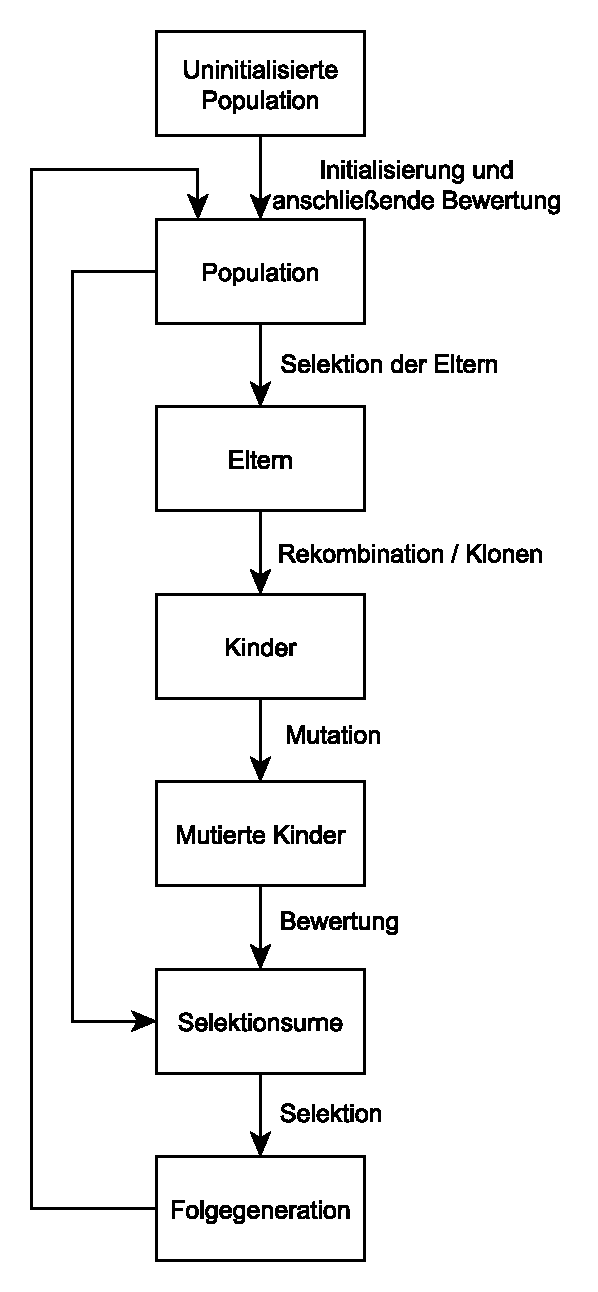
\includegraphics[width=0.4\textwidth]{img/ablauf_einer_evolution.pdf}
\caption[Ablauf einer Evolution]{Ablauf einer Evolution\protect\footnotemark}
\label{fig:ablauf_einer_evolution}
\end{figure}
\footnotetext{\url{http://www.evocomp.de/themen/evolutionsalgorithmen/pic/Evolutionsalgorithmen_Ablauf.gif}}

Zu Beginn werden Parameterkonfigurationen, sogenannte \enquote{Individuen}, zufällig aufgebaut.
Anschließend werden daraus Eltern nach einem festgelegten Verfahren bestimmt, deren Informationen nach einem Klonvorgang bzw. einer Rekombination mehrerer Eltern an Kinder weitergegeben werden.
Zu einer gewissen Wahrscheinlichkeit werden die nachkommenden Individuen mutiert, bevor sie abschließend anhand einer Qualitätsfunkton nach deren \enquote{Fitness} für die nächste Generation selektiert werden.
Die qualitativ hochwertigsten Nachkommen dienen in der nächsten Iteration als Eltern.
Werden mehrere Individuen über den evolutionären Prozess hinweg beibehalten, spricht man bei einer Sammlung von Individuen von einer \enquote{Population}.

Eine Evolutionsstrategie gewährleistet keinen stetigen Qualitätsfortschritt. Oftmals kann eine Population an einem lokalen Maximum, als an einer suboptimalen Lösung, festhängen. Rückschritte in der Entwicklung sind auch möglich und hängen auch von der gewählten \enquote{Schrittweite} ab. Diese bestimmt, in welchem Maß die Parameterwerte eines von mindestens einem Elter stammenden Nachkommens angepasst werden.

\setlistingtopseudocode

\begin{lstlisting}[caption=Grundlegende Evolutionsstrategien, firstnumber=1, captionpos=b, label=code:standard_es]
iterationsLimit <- x $\in \mathbb{N}$
generationszaehler <- 0
population <- buildPopulation()
while fitness(selectSingleBest(population)) nicht zufriedenstellend or generationszaehler < iterationslimit
	eltern <- select(population)
	kinder <- clone(eltern)
	kinder <- mutate(kinder)
	urne <- population + kinder
	population <- selectMultipleBest(urne)
loesung <- selectSingleBest(population)
\end{lstlisting}

\subsection{Aufbau der Ausarbeitung}

Nachdem die allgemeine Thematik im Grundsatz bekannt ist, wird im nächsten Abschnitt auf die Kodierung der Individuen eingegangen. Anschließend werden grundlegende, unterschiedliche Evolutionsstrategien behandelt, wobei jeweils ein zugehöriger Pseudocode-Abschnitt zur schnellen Umsetzung der jeweiligen Strategie dienen soll.

Dabei werden die Unterschiede zwischen den Evolutionsstrategien angesprochen. Hauptmerkmal der Evolutionsstrategien ist die Evolution. In Hinblick darauf wird die $\frac{1}{5}$-Regel als Grundtechnik und die mutative Schrittweitensteuerung zur Anpassung der Evolution detailliert aufgefasst.

%--
\section{Codierung}
% Was ist eine Codierung
Unter der Codierung eines Individuums versteht man Informationsketten, mit denen sich Individuen eindeutig voneinander unterscheiden lassen.
% Codierung in der Natur
Die Gene eines Menschen können so als dessen Codierung angesehen werden.
% Codierung bei den Evolutionsstrategien
Bei den Evolutionsstrategien wurde auf eine komplizierte Codierung verzichtet und dafür eine sehr kure Codierungsform eingesetzt. Die relevanten Erbinformationen von Individuen werden durch Vektoren reeller Zahlen dargestellt \cite{}. Diese Vektoren werden Chromosome genannt. Jedes Individuum hat ein solches Chromosom.
Eine Menge an Individuen bildet eine Population. Diese Codierungsweise wird in der Grafik \ref{fig:codierung} dargestellt. Darin ist zu sehen, wie eine Menge an Individuuen eine Population bildet. Die Individuen sind als Männchen verbildlicht. Darüber hinaus ist ein Chromosomausschnnitt abgebildet.
Die Wahl für diese Codierungsvariante lässt sich darin begründen, dass die Evolutionsstrategien zu Beginn für ingenieurstechnische Optimierungen verwendet wurden \cite{}.
In diesem Aufgabenfeld werden optimale Systemparameter gesucht. Diese lassen sich sehr gut als Vektoren reeler Zahlen abbilden.
Der durch die Evolutionsstrategien gewählte Codierungansatz wird als phänotypisch orientiert bezeichnet \cite{}. Das bedeutet, dass im Gegensatz zu einer genotypischen Orientierung, die Eigenschaft des Individuums betrachtet wird und nicht die Chromosome selbst.
Die Eigenschaft des Individuums kann durch Qualitätsfunktionen berechnet werden.

\begin{figure}[!htb]
	\centering
	\includegraphics[width=1.\textwidth]{img/codierung/codierung.png}
	\caption{Grafische Darstellung einer Population, von Individuen und eines Chromosoms.}
\label{fig:codierung}
\end{figure}



\section{Typisches Aussehen einer Evolutionsstrategie}
%1. Obwohl viel Variation, erkannte Rechenberg Abschnitte die häufig wiederzufinden sind
Evolutionsstrategien können einen sehr hohen Grad an Variation aufweisen. Je nach Aufgabengebiet unterscheiden sich die Verfahren stark.
Rechenberg konnte allerdings Verfahrensabschnitte benennen, aus denen sich typischerweise Evolutionsstrategien zusammensetzen.
Diese Verfahrensabschnitte bilden die Rechenbergsche Grafik-Notation \cite[S.~144-146]{schoeneburg}. In diesem Kapitel wird das typische Aussehen einer Evolutionsstrategie mithilfe der Rechenberg'schen Grafik-Notation erläutert.

\subsection{Rechenbergsche Grafik-Notation}
%2. Die Rechenbergnotation erklären
Die Rechenbergs'chen Grafik-Notation orientiert sich an Spielkarten und kommt bereits mit zehn verschiedenen Symbolen aus.
Die gesamte Rechenberg'sche Grafik-Notation ist in Abbildung \ref{fig:rechenberg} zu sehen. Abläufe, die in einer natürlichen Evolution stattfinden, finden sich in dieser Notation wieder.
Die Komplexität der Evolutionsstrategien wird durch deren Kombination erreicht. Zudem ist es möglich, die Populationen innerhalb weiterer Populationen endlos zu schachteln.\\
Die grundlegende Einheit in dieser Notation ist das Individuum. Dieses wird mit einer Spielkarte (\ref{fig:individuum}) symbolisiert. Die schwarzen Punkte auf der Karte sollen dabei die Chromosome darstellen.
Eine Population setzt sich aus mehreren Individuen zusammen. Daher wählte Rechenberg einen Stapel (\ref{fig:population}) an Spielkarten für dessen Darstellung. Zur Verarbeitung der Individuen und der Populationen definierte Rechenberg acht weitere Symbole.
Für die Verarbeitung von Populationen stehen Methoden bereit, mit denen eine Teilmenge an Individuen ausgewählt werden kann. Dazu gibt es die gleichverteilte Auswahl \ref{fig:auswahl_gleichverteilt} und die Auswahl nach einer Qualitätsfunktion \ref{fig:auswahl_qualitaetsfunktion}.
Der Kreis um die Population soll eine Urne symbolisieren, aus der Individuen gezogen werden. Bei der gleichverteilten Auswahl hat jedes Individuum die gleiche Wahrscheinlichkeit aus der Urne gezogen zu werden. Bei der Auswahl nach einer Qualitätsfunktion entscheidet die Qualität der Individuen über die Wahrscheinlichkeit, ausgewählt zu werden.
Je höher die Qualität des Individuums, desto höher die Wahrscheinlichkeit. Auch das Verwenden von isolierten Populationen ist mit der Rechenberg'schen Grafik-Notation möglich. Dafür gibt es das Populationssymbol \ref{fig:population_isoliert}, welches mit einem Stacheldraht eingegrenzt ist. Dieses Symbol kann hilfreich sein, wenn mehrere voneinander isolierte Populationen existieren sollen, welche sich unabhängig voneinander entwickeln.\\
Alle weiteren Notationssymbole sind Funktionen, die auf einzelne Individuen angewendet werden. Um ein Individuum zu duplizieren, wird das Symbol \ref{fig:duplikation} verwendet. Soll das duplizierte Individuum mutieren, so ist das Symbol \ref{fig:mutation} zu verwenden. Zeigt, wie auf dem Symbol \ref{fig:bewertung}, ein Pfeil mit einem Q auf ein Individuum, so wird eine Qualitätsfunktion auf das Individuum angewendet. Damit auch die Fortpflanzung mehrerer Individuen zu einem neuen Individuum möglich ist, gibt es eigens das Notationssymbol \ref{fig:rekombination} für die Rekombination. Rekombination bedeutet, dass durch eine Kombination der Elternchromosome ein neues Kindindividuum als Nachkomme erzeugt wird.
Es kann auch notwendig sein, die genotypischen Merkmale in phänotypische Merkmale umzuwandeln. Dies ist dann notwendig, wenn über die Geninformationen nicht direkt eine Aussage über die Qualität des Individuums getroffen werden kann. In diesen Fällen müssen die Merkmale, die sich aus den Geninformationen ergeben, in einer Funktion berechnet werden. Dieses Umwandeln wird mit dem Symbol der phänotypischen Realisation \ref{fig:phaenotypische_realisation} dargestellt.

\begin{figure}[!htb]
\begin{subfigure}{.3\textwidth}
	\centering
	\includegraphics[width=.4\linewidth]{img/rechenberg_notation/individuum.png}
	\caption{Individuum}
	\label{fig:individuum}
\end{subfigure}
\begin{subfigure}{.3\textwidth}
	\centering
	\includegraphics[width=.5\linewidth]{img/rechenberg_notation/population.png}
	\caption{Population}
	\label{fig:population}
\end{subfigure}
\begin{subfigure}{.3\textwidth}
	\centering
	\includegraphics[width=.7\linewidth]{img/rechenberg_notation/auswahl_gleichverteilt.png}
	\caption{Gleichverteilte Auswahl}
	\label{fig:auswahl_gleichverteilt}
\end{subfigure}

\begin{subfigure}{.3\textwidth}
	\centering
	\includegraphics[width=.7\linewidth]{img/rechenberg_notation/auswahl_qualitaetsfunktion.png}
	\caption{Auswahl mit einer Qualitätsfunktion}
	\label{fig:auswahl_qualitaetsfunktion}
\end{subfigure}
\begin{subfigure}{.3\textwidth}
	\centering
	\includegraphics[width=.7\linewidth]{img/rechenberg_notation/population_isoliert.png}
	\caption{Isolierte Population}
	\label{fig:population_isoliert}
\end{subfigure}
\begin{subfigure}{.3\textwidth}
	\centering
	\includegraphics[width=.7\linewidth]{img/rechenberg_notation/duplikation.png}
	\caption{Duplikation}
	\label{fig:duplikation}
\end{subfigure}

\begin{subfigure}{.3\textwidth}
	\centering
	\includegraphics[width=.7\linewidth]{img/rechenberg_notation/mutation.png}
	\caption{Mutation}
	\label{fig:mutation}
\end{subfigure}
\begin{subfigure}{.3\textwidth}
	\centering
	\includegraphics[width=.4\linewidth]{img/rechenberg_notation/bewertung.png}
	\caption{Bewertung}
	\label{fig:bewertung}
\end{subfigure}
\begin{subfigure}{.3\textwidth}
	\centering
	\includegraphics[width=.7\linewidth]{img/rechenberg_notation/rekombination.png}
	\caption{Rekombination}
	\label{fig:rekombination}
\end{subfigure}

\begin{subfigure}{.3\textwidth}
	\centering
	\includegraphics[width=.5\linewidth]{img/rechenberg_notation/phaenotypische_realisation.png}
	\caption{Phänotypische Realisation}
	\label{fig:phaenotypische_realisation}
\end{subfigure}
\caption[Rechenbergsche Grafik-Notation]{Rechenbergsche Grafik-Notation \cite[S.~145]{schoeneburg}}
\label{fig:rechenberg}
\end{figure}


% 3. Typische Reihenfolge der Abschnitte kurz zeigen. Aber auch klar machen das das ganze extrem variieren kann
\subsection{Aufbau einer Evolutionsstrategie}

Die Rechenberg'sche Grafik-Notation wird im folgenden zur Modellierung des Aufbaus von Evolutionsstrategien verwendet. In Abbildung \ref{fig:flowchart_es} ist ein Flussdiagramm zu sehen, das den Ablauf einer Evolutionsstrategie abstrakt darstellt.

Zu Beginn wird eine Startpopulation gebildet. Für diese Population können die Chromosome der einzelnen Individuen zufällig gewählt werden. Aus dieser Population wird anschließend eine Teilmenge gebildet. Diese Teilmenge kann als Elternpopulation bezeichnet werden, denn die Nachkommen werden aus diesen Individuen erzeugt. Bei den Evolutionsstrategien hat jedes Individuum die selbe Wahrscheinlichkeit für die Elternpopulation ausgewählt zu werden \cite[S.~220]{schoeneburg}. Eine Auswahl über deren Qualität findet nicht statt. Die Nachkommen der Elternpopulation werden erzeugt, indem die Eltern dupliziert werden. Die Generation der Nachkommen kann auch durch eine Kombination der Chromosome von mehreren Elternindividuen gebildet werden. Zu einer gewissen Wahrscheinlichkeit werden die Chromosome der Individuen anschließend mutiert. Somit individualisieren sich die Nachkommen in ihrer Eigenschaft. 
Nach der Mutation hat sich aus der Elternpopulation eine Population an Nachkommen gebildet. Aus der Startpopulation und der Nachkommendenpopulation wird anschließend über eine Selektion eine neue Population erzeugt, welche die Grundlage für die nächste Evolutionsgeneration dient. Die Selektion beruht, anders als bei der Bildung der Elternpopulation, auf Basis einer Qualitätsfunktion, die auf das vorliegende Problem angepasst sein muss, um eine sinnvolles Selektionsverfahren zu ermöglichen.

Bei der Auswahl der Individuen gibt es verschiedene Ansätze, die im Laufe dieser Ausarbeitung näher beschrieben werden. Genügt die Qualität der Population noch nicht den gewünschten Ansprüchen, so kann kann die gebildete Population für einen weiteren Evolutionsschritt verwendet werden.
Das grundlegende Verfahren ist im Pseudocode \ref{lst:es} übersichtlich aufgeführt. Die wenigen notwendigen Schritte aus denen sich Evolutionsstrategien zusammensetzen verdeutlichen, dass es Rechenberg nicht darum ging, die Evolution perfekt nachzubilden, sondern diese lediglich als Anfangspunkt einer technischen Umsetzung zu betrachten. Aus diesem Grund sind in den nächsten Kapiteln dieser Ausarbeitung Evolutionsstrategien zu sehen, die sich zwar an der natürlichen Evolution orientieren, diese aber nicht realitätsnah abzubilden versuchen.

\pagebreak

\begin{lstlisting}[caption={Grundlegende Evolutionsstrategie}, firstnumber=1, captionpos=b, label=lst:es]
algorithm ES()
	iterationsLimit <- x $\in \mathbb{N}$
	wunschqualitaet <- y $\in \mathbb{R}$
	generationszaehler <- 0
	population <- baue_population()
	while qualitaet(population) < wunschqualitaet or generationszaehler < iterationslimit
		generationszähler <- generationszähler + 1
		eltern <- elternSelektion(population)
		kinder <- duplikation(eltern) // oder: rekombination(eltern)
		kinder <- mutation(kinder)
		population <- selektion(eltern + kinder, size(population), qualitaet)
	loesung <- bestenSelektion(population)
	return loesung
\end{lstlisting}

\begin{figure}[!htb]
	\centering
	\includegraphics[height=\textheight, keepaspectratio]{img/typisches_aussehen/es_grafik.png}
	\caption{Flussdiagramm einer Evolutionsstrategie}
	\label{fig:flowchart_es}
\end{figure}

%-- steuerung der evolution

\section{Steuerung der Evolution}

In diesem Kapitel werden die wesentlichen Evolutionsstrategien sowie deren Handlungsabfolge mithilfe von Pseudocode-Abschnitten näher beschrieben.

\subsection{$(1+1)$-ES}

Die $(1+1)$-Evolutionsstrategie gilt als einfachste Form der ES. Bereits damit hat Rechenberg 1964 die optimale Einstellung von Gelenkwinkeln einer Gelenkplatte berechnen lassen.

Es handelt sich um eine zweigliedrige Strategie, bei dem es in jeder Evolutionsiteration genau ein Ur-Individuum bzw. Elternindividuum gibt, welches der Erzeugung von genau einem nachkommenden Individuum (Kindindividuum) dient. Dabei wird der Ausgangsvektor analog zum biologischen Prozess der DNS-Selbstverdopplung dupliziert. Das zweite, bislang wertgleiche, Individuum wird anschließend zufällig, allerdings nicht willkürlich, modifiziert. Meist wird ein kleiner reeller Wert auf jeden Vektorparameter addiert.

Die beiden, nun unterschiedlichen, Individuen werden nach dem Prinzip \enquote{survival of the fittest} bewertet.
Anhand des Outputs einer Qualitätsfunktion wird verglichen, welcher der beiden Individuen das angemessenere ist und anschließend zur Fortführung der Evolution selektiert werden soll.
Umgangssprachlich spricht man von einem \enquote{Sterben der Schwachen} und einem \enquote{Überleben der Starken}.
Bei gleicher Qualitätsbewertung wird ein Individuum zufällig selektiert.
Als Zeitmaß für die Evolutionsiteration dient die \enquote{Generation}, wobei die Generation $G_0$ die Ausgangsgeneration mit einem Ausgangsindividuum bildet. Die Selektion aus dessen Elterindividuum sowie dessen Nachkomme bildet die Generation $G_1$ und so weiter.

Aus diesem Vorgehen bedeutet die Namensgebung "$(1+1)$-ES": Ein Elternindividuum wird zusammen mit einem nachkommenden Individuum für die Selektion betrachtet.

In diesem Fall wird das Erbgut ausschließlich über die Mutation verändert. Es gibt keine sexuelle Rekombination des Erbgutes.

Es handelt sich zwar um eine grundlegende und kompakte Form der Abbildung von Evolutionsmechanismen, jedoch können auch hierbei in Kombination mit der adaptiven Schrittweitenregelung zur Mutation der Nachkommen (\textit{siehe Kapitel \ref{sec:mutation}}) sinnvolle Anwendungen entstehen.

Abbildung \ref{fig:1_und_1_es} veranschaulicht den Ablauf anhand der Rechenberg'schen Grafik-Notation. Da bereits bei dieser einfachen Evolutionsstrategie eine recht flächendeckende Veranschaulichung benötigt wird, welche mit steigender Komplexität wesentlich schwerer zu überblicken ist, wurde auf eine Veranschaulichung der weiteren Evolutionsstrategien verzichtet. 

\begin{figure}[H]
\centering
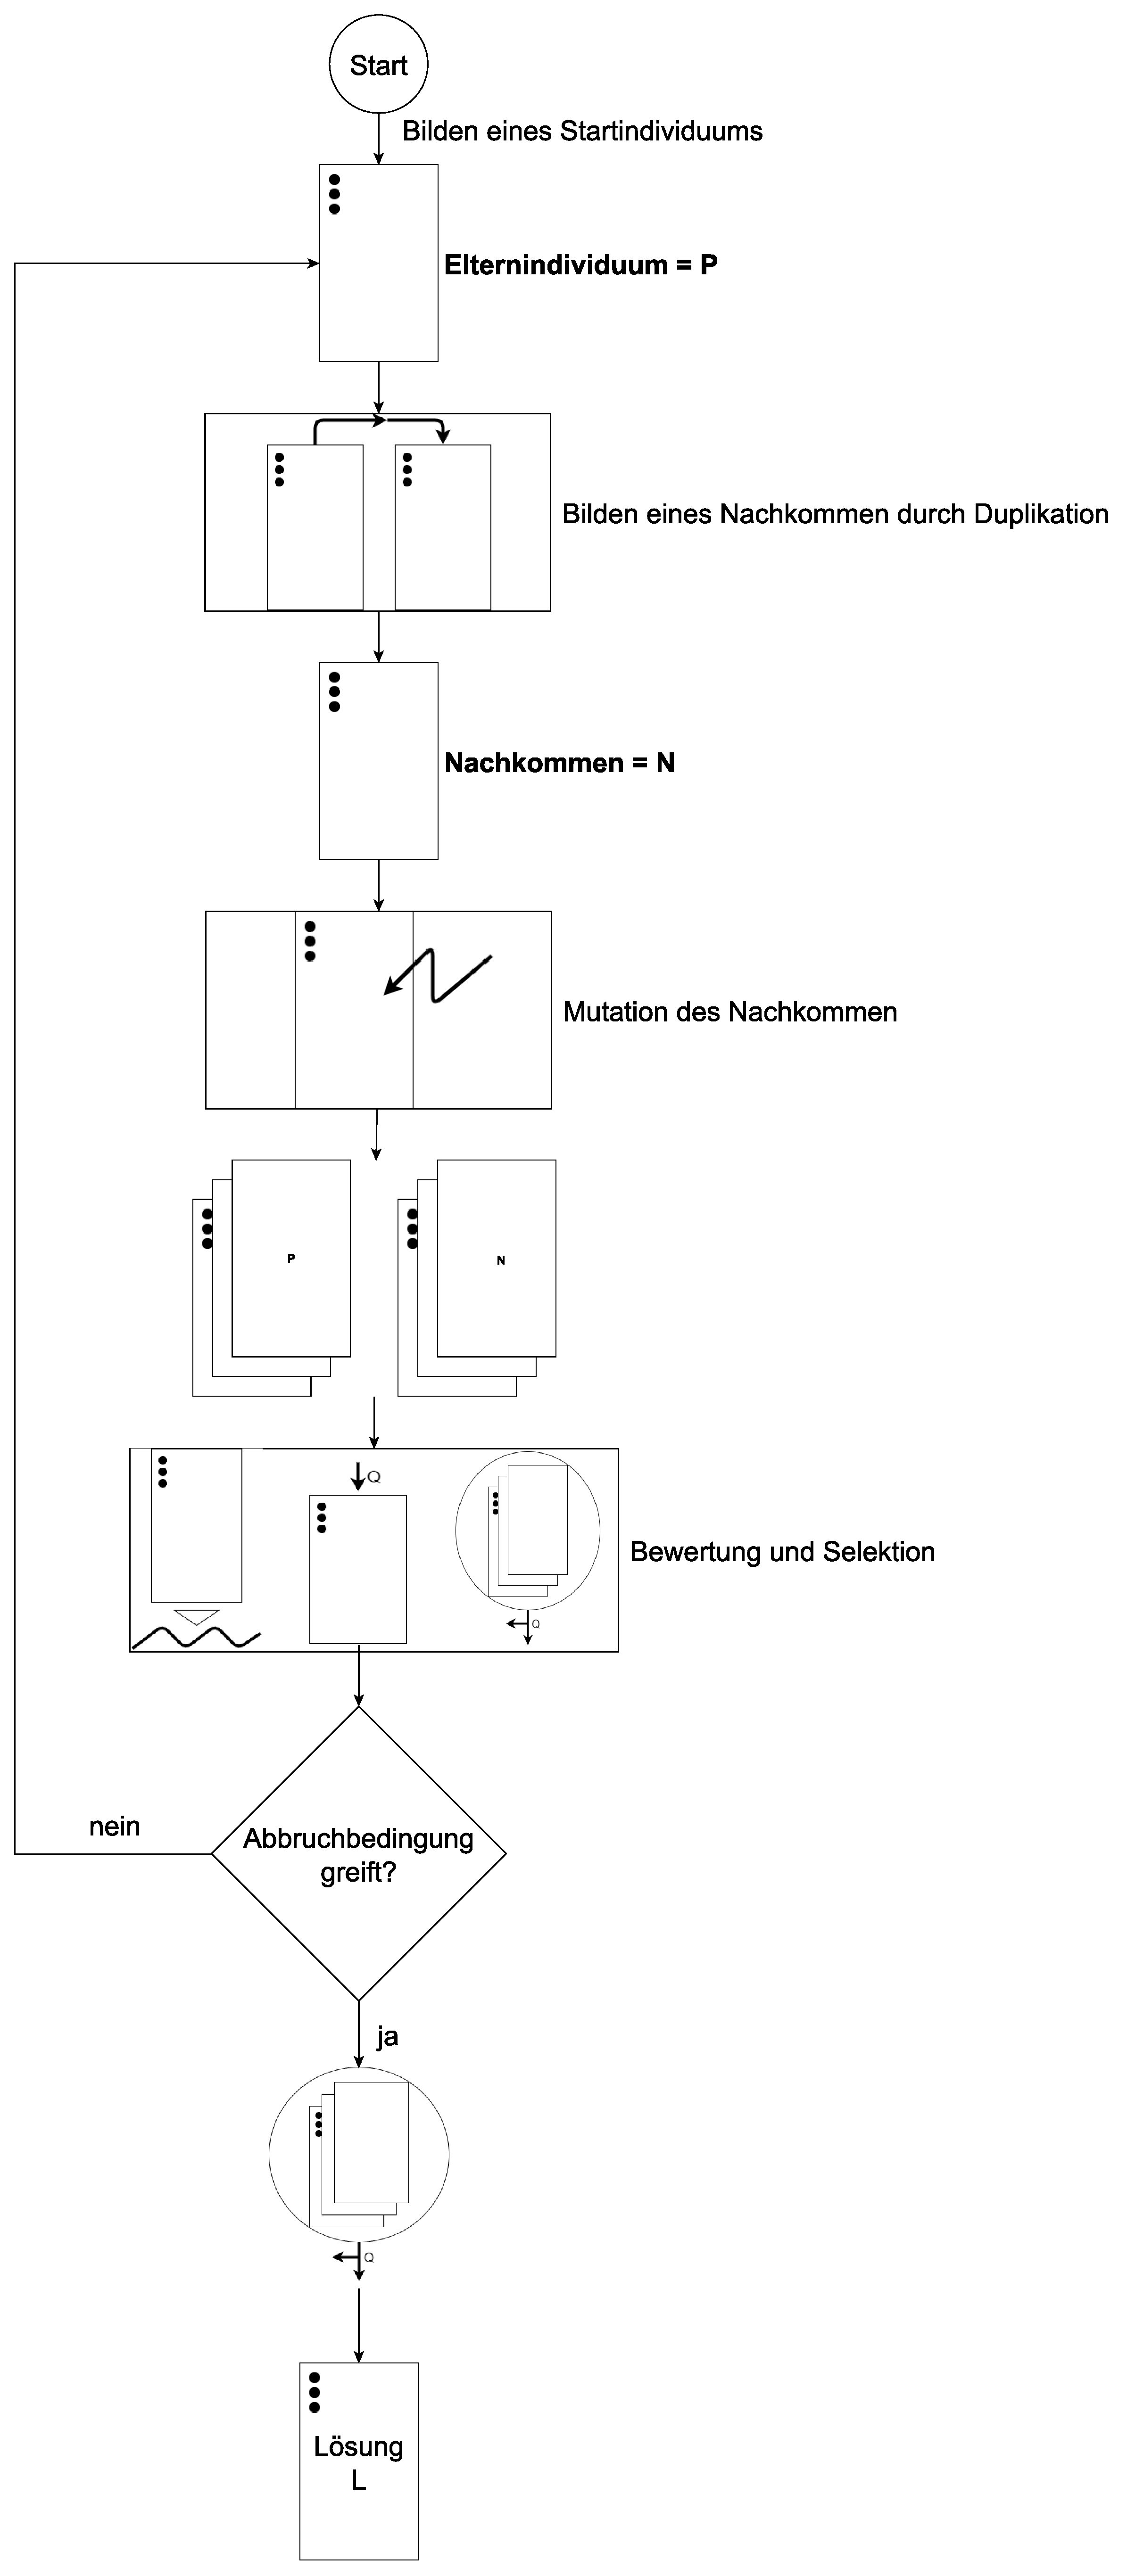
\includegraphics[width=0.4\textwidth]{img/1_und_1_es.pdf}
\caption{$(1+1)$-ES}
\label{fig:1_und_1_es}
\end{figure}

Folgender Pseudocode-Abschnitt \ref{lst:1_und_1_es} verdeutlicht die grundlegende Vorgehensweise. Während die grüne Zeilenmarkierung den Beginn der wesentlichen Evolutionsstrategie hervorhebt, hebt eine blaue Markierung die nun relevanten Unterschiede im Vergleich zur jeweils vorigen Evolutionsstrategie hervor.

\begin{lstlisting}[caption={$(1+1)$-Evolutionsstrategie}, firstnumber=1, captionpos=b, label=lst:1_und_1_es]
<@\colorcodeline{algorithm baue\_individuum(n)}@>
	individuum <- []	
	for _ <- 1,...,n
		individuum <- individuum + zufälliges $x \in \mathbb{R}$
	return individuum
	
<@\colorcodeline{algorithm qualitaet(individuum | population)}@>
	// problemspezifische Qualitätsfunktion

	
<@\colorcodeline{algorithm duplikation(individuum[1,...,n])}@>
	klon <- []
	for i <- 1,...,n
		klon <- klon + individuum[i]
	return klon
	
<@\colorcodeline{algorithm selektion(individuen[1,...,m], $\mu$, qualitaetsfunktion)}@>
	sortierteIndividuen <- sortiereAbsteigend(individuen, qualitaetsfunktion)
	besteIndividuen <- []
	for i <- 1,...,$\mu$
		besteIndividuen <- besteIndividuen + sortierteIndividuen[i]
	return besteIndividuen

<@\colorcodealgorithm{algorithm $(1+1)$-ES()}@>
	iterationsLimit <- x $\in \mathbb{N}$
	generationszaehler <- 0
	wunschqualitaet <- y $\in \mathbb{R}$
	individuengroesse <- n $\in \mathbb{N}$
	<@\colorcodeline{individuum <- baue\_individuum(individuengroesse)}@>
	while qualitaet(individuum) < wunschqualitaet and generationszaehler < iterationslimit
		generationszaehler <- generationszaehler + 1
		elter <- individuum
		<@\colorcodeline{kind <- duplikation(elter)}@>
		kind <- mutation(kind)
		individuum <- selektion([elter, kind], 1, qualitaet)
	loesung <- individuum
	return loesung
\end{lstlisting}

\subsection{$(\mu + \lambda)$-ES}

Mit der $(\mu + \lambda)$-Evolutionsstrategie wird die vorige $(1+1)$-ES in einer allgemeineren Form übertragen.
Dabei gilt:

\begin{equation}
1 \le |Eltern| \le |Nachkommen| \Leftrightarrow 1 \le \mu \le \lambda
\end{equation}
\myequations{Beziehung zwischen Eltern und Kinder}

Es müssen aus den $\mu$ Eltern also $\lambda$ Nachkommen erzeugt werden, wobei es mindestens genau so viele Nachkommen wie Eltern geben muss.
Alle Individuen werden gemeinsam für eine Selektion der besten Individuen betrachtet, sowohl die Eltern als auch die Kinder.
Somit können einige Elternindividuen über mehrere Generationen hinweg bestehen, sofern sie sich einem im Vergleich hohen Qualitätswert zuordnen lassen.

Das \enquote{+} der $(\mu + \lambda)$-Notation lässt sich somit als Vereinigung sowohl der Eltern als auch der Nachkommen lesen, die abschließend gemeinsam selektiert werden.

Werden mehrere Nachkommen erzeugt als es Eltern gibt, also:

\begin{equation}
|Nachkommen| > |Eltern| \Leftrightarrow \lambda > \mu
\end{equation}
\myequations{Bedingung für die Mehrfachselektion von Eltern}

dann müssen einige Eltern mehrfach zur Erzeugung eines Nachkommens ausgewählt werden.
Von allen Individuen werden anschließend die $|Eltern| = \mu$ besten als Basis für die nächste Generation ausgewählt. Die Größe der Elternpopulation bleibt somit immer konstant. Da die Eltern \textbf{und} die Nachkommen bewertet werden und zur Selektion bereitstehen, nimmt die Qualität des besten Individuums der nächsten Population im Vergleich zur vorigen niemals ab.

Algorithmisch sind die Anzahlen der Nachkommen und der Eltern folglich nun frei wählbar, wobei die Anzahl der zu erzeugenden Nachkommen anhand der erläuterten Bedingung mindestens so groß wie die Anzahl der Elternindividuen sein muss. Dies wird in Pseudocode \ref{lst:mu_und_lambda_es} dargestellt.

\begin{lstlisting}[caption={$(\mu + \lambda)$-Evolutionsstrategie}, firstnumber=1, captionpos=b, label=lst:mu_und_lambda_es]
<@\colorcodeline{algorithm baue\_population($\mu$, n)}@>
	population <- []
	for i <- 1,...,$\mu$
		individuum <- baue_individuum(n)
		population <- population + individuum
	return population
	
<@\colorcodeline{algorithm elternSelektion(population[1,...,$\mu$], $\lambda$)}@>
	individuen <- []
	for _ <- 1,...,$\lambda$
		idx <- zufälliges x $\in \{1,...,\mu\}$
		individuum <- population[idx]
		individuen <- individuen + individuum
	return individuen
	

<@\colorcodeline{algorithm duplikation(individuen[1,...,$\mu$], n)}@>
	klone <- []
	for i <- 1,...,$\mu$
		klon <- []
		for j <- 1...n
			klon <- klon + individuen[i][j]
		klone <- klone + klon
	return klon
	
<@\colorcodeline{algorithm bestenSelektion(population[1,...,$\mu$])}@>
	beste_loesung <- []
	for i <- 1,...,$\mu$
		individuum <- population[i]
		if qualitaet(individuum) > qualitaet(beste_loesung)
			beste_loesung <- individuum
	return beste_loesung
	

<@\colorcodealgorithm{algorithm $(\mu + \lambda)$-ES()}@>
	iterationsLimit <- x $\in \mathbb{N}$
	generationszaehler <- 0
	anzahl_eltern <- $\mu \ge 1$
	anzahl_kinder <- $\lambda \ge$ anzahl_eltern
	wunschqualitaet <- y $\in \mathbb{R}$
	individuengroesse <- n $\in \mathbb{N}$
	<@\colorcodeline{population <- baue\_population($\mu$, individuengroesse)}@>
	while qualitaet(population) < wunschqualitaet and generationszaehler < iterationslimit
		generationszaehler <- generationszaehler + 1
		<@\colorcodeline{eltern <- elternSelektion(population, anzahl\_kinder)}@>
		<@\colorcodeline{kinder <- duplikation(eltern, individuengroesse)}@>
		kinder <- mutation(kinder)
		<@\colorcodeline{population <- selektion(eltern + kinder, $\mu$, qualitaet)}@>
	loesung <- bestenSelektion(population)
	return loesung
\end{lstlisting}

\subsection{$(\mu, \lambda)$-ES}

Als weitere Evolutionsstrategie gibt es die Komma-Notation, welche von Schwefel in seiner Dissertation 1975 eingeführt wurde. Bei $(\mu + \lambda)$-ES kann das beste Individuum nicht vergessen gehen, da in jeder Iteration alle Individuen bei der Selektion berücksichtigt werden. Auf den ersten Blick klingt dies nach einem wünschenswerten Effekt, jedoch können negative Auswirkungen die Folge sein, wenn es sich dabei um ein lokales Optimum laut der Qualitätsfunktion handelt.
Das globale Optimum und somit die optimale Lösung des Problems wird daraufhin häufig nicht mehr gefunden.

Schwefels $(\mu, \lambda)$-ES nutzt einen veränderten Selektionsmechanismus:
Die Elternindividuen werden bei der abschließenden Selektion nicht mehr berücksichtigt und somit vergessen. Es werden lediglich $|Eltern| = \mu$ der $|Nachkommen| = \lambda$ Nachkommen für die nächste Generation ausgewählt.

Insofern handelt es sich um ein einigermaßen naturgetreues Modell der Evolution. Kein Individuum ist mehr unsterblich. Allerdings sterben die Individuen direkt nach einer Generation. Aufgrund dessen sind allerdings auch Rückschritte in der Evolution möglich.

Anhand des folgenden Pseudocodes \ref{lst:mu_nur_lambda_es} ist zu erkennen, dass sich nur die abschließende Selektion verändert hat.

\begin{lstlisting}[caption={$(\mu, \lambda)$-Evolutionsstrategie}, firstnumber=1, captionpos=b, label=lst:mu_nur_lambda_es]
<@\colorcodealgorithm{algorithm $(\mu , \lambda)$-ES()}@>
	iterationsLimit <- x $\in \mathbb{N}$
	generationszaehler <- 0
	anzahl_eltern <- $\mu \ge 1$
	anzahl_kinder <- $\lambda \ge$ anzahl_eltern
	wunschqualitaet <- y $\in \mathbb{R}$
	individuengroesse <- n $\in \mathbb{N}$
	population <- baue_population($\mu$, individuengroesse)
	while qualitaet(population) < wunschqualitaet and generationszaehler < iterationslimit
		generationszaehler <- generationszaehler + 1
		eltern <- elternSelektion(population, anzahl_kinder)
		kinder <- duplikation(eltern, individuengroesse)
		kinder <- mutation(kinder)
		<@\colorcodeline{population <- selektion(kinder, $\mu$, qualitaet)}@>
	loesung <- bestenSelektion(population)
	return loesung
\end{lstlisting}

\subsection{$(\mu \# \lambda)$-ES}

Die $(\mu \# \lambda)$-Notation bedeutet lediglich, dass das abschließende Selektionsschema zur Bildung der Basispopulation für die nächste Generation keine Rolle spielt.
Es werden aus den $\mu$ Eltern $\lambda$ Nachkommen erzeugt. Die Selektion kann, wie in Pseudocode \ref{lst:mu_hash_lambda_es} dargestellt, beliebig durchgeführt werden.

\begin{lstlisting}[caption={$(\mu \# \lambda)$-Evolutionsstrategie}, firstnumber=1, captionpos=b, label=lst:mu_hash_lambda_es]
<@\colorcodealgorithm{algorithm $(\mu \# \lambda)$-ES()}@>
	iterationsLimit <- x $\in \mathbb{N}$
	generationszaehler <- 0
	anzahl_eltern <- $\mu \ge 1$
	anzahl_kinder <- $\lambda \ge$ anzahl_eltern
	wunschqualitaet <- y $\in \mathbb{R}$
	individuengroesse <- n $\in \mathbb{N}$
	population <- baue_population($\mu$, individuengroesse)
	while qualitaet(population) < wunschqualitaet and generationszaehler < iterationslimit
		generationszaehler <- generationszaehler + 1
		eltern <- elternSelektion(population, anzahl_kinder)
		kinder <- duplikation(eltern, individuengroesse)
		kinder <- mutation(kinder)
		<@\colorcodeline{population <- selektion(eltern + kinder, $\mu$, qualitaet)}@>
		<@\colorcodeline{// oder population <- selektion(kinder, $\mu$, qualitaet)}@>
	loesung <- bestenSelektion(population)
	return loesung
\end{lstlisting}

\subsection{Selektionsdruck und Populationswellen}

$(\mu \# \lambda)$-ES erlauben eine einfache Beschreibung und Simulation des Selektionsdrucks innerhalb einer Population als auch von Populationswellen.
Bei dem Selektionsdruck handelt es sich um einen Quotienten $s$, welcher besagt, in welchem Verhältnis die Anzahl der Elternindividuen zu den Nachkommen stehen.

\begin{equation}
\begin{aligned}
s = \frac{\mu}{\lambda} \\
0 < s \le 1
\end{aligned}
\end{equation}
\myequations{Selektionsdruck}

Je größer die Anzahl der erzeugten Nachkommen $\lambda$ im Verhältnis zu den Eltern $\mu$, desto mehr Individuen werden erzeugt, als in die nächste Generation übernommen werden können.
Liegt $\lambda$ dicht bei $\mu$, so werden nur wenige Individuen aufgrund einer schlechten Bewertung aussortiert und folglich nicht in die nächste Generation übernommen.
Der Druck, der auf einem Individuum lastet, um selektiert zu werden und folglich zu überleben und in die nächste Generation aufgenommen zu werden wächst, je mehr Auswahl es bei der Selektion gibt.
Somit steht $0$ für einen starken und $1$ für einen schwachen Selektionsdruck.

Unter Populationswellen versteht man eine Anpassung der Parameter $\mu$ und $\lambda$ einer Evolutionsstrategie über Generationen hinweg. Insofern dient eine unterschiedliche Anzahl an Eltern der Erzeugung einer unterschiedlichen Anzahl an Nachkommen.
Um einen gleichbleibenden Selektionsdruck zu erzielen, müssen die Parameter $\mu$ und $\lambda$ stets in gleichem Verhältnis zueinander stehen und können nur eingeschränkt angepasst werden.

In Bezug auf die Biologie sind periodisch und zyklische Variationen des Selektionsdrucks besonders interessant.

\subsection{$(\mu / p \# \lambda)$-ES}

In den bislang genannten Evolutionsstrategien wurde die sexuelle Rekombination nicht berücksichtigt. Es fand lediglich ein Klonverfahren eines Elternindividuums zur Erzeugung von Nachkommen statt.
Diese wird mit der $(\mu / p \# \lambda)$-ES nun betrachtet.
In den Grundzügen baut diese Evolutionsstrategie auf den vorigen auf, jedoch gibt es nun einen Unterschied bei der Erzeugung von nachkommenden Individuen.
Anstatt einzelne Elternindividuen werden dazu nun Gruppen von Elternindividuen herangezogen.
Das $p$ entspricht somit der Anzahl der Elemente einer Gruppe zur Erzeugung eines Nachkommens.
Die Nachkommen entstehen nicht mehr nur aus der Kopie eines Elters, sondern aus einer gemeinsamen Kombination aller beteiligten Eltern.

\enquote{\textbackslash} dient als Vermischungssymbol für die Rekombination in der Notation.

Standardmäßig werden dazu zwei Eltern ($p = 2$) genutzt.
In diesem Fall wird für jeden Parameter einzeln per gleichverteilten Zufall entschieden, welche Parameterausprägung wessen Elternindividuums nun weiter vererbt wird.
Aus den beiden resultierenden Individuen wird per Zufall nur einer zur finalen Erzeugung ausgewählt.
Pseudocode \ref{lst:mu_p2_lambda_es} verdeutlicht den Vorgang.

\begin{lstlisting}[caption={$(\mu / p \# \lambda)$-Evolutionsstrategie mit $p = 2$}, firstnumber=1, captionpos=b, label=lst:mu_p2_lambda_es]
<@\colorcodeline{algorithm gruppenSelektion(population[1,...,$\mu$], $\lambda$, p)}@>
	gruppen <- []
	for i <- 1,...,$\lambda$
		gruppe <- []
		for j <- 1,...,p
			idx <- zufälliges $x \in \{1,...,\mu\}$
			individuum <- population[idx]
			gruppe <- gruppe + individuum
		gruppen <- gruppen + gruppe
	return gruppen

<@\colorcodeline{algorithm rekombination(gruppen[1,...,$\lambda$], p, n)}@>
	individuen <- []
	for i <- 1,...,$\lambda$
		individuum <- []
		gruppenindividuen <- gruppen[i]
		for j <- 1,...,n
			idx <- zufälliges $x \in \{1,...,p\}$
			gruppenindividuum <- gruppenindividuen[idx]
			individuum <- individuum + gruppenindividuum[j]
		individuen <- individuen + individuum
	return individuen

<@\colorcodealgorithm{algorithm $(\mu / p \# \lambda)$-ES()}@>
	iterationsLimit <- x $\in \mathbb{N}$
	generationszaehler <- 0
	anzahl_eltern <- $\mu \ge 1$
	anzahl_kinder <- $\lambda \ge$ anzahl_eltern
	wunschqualitaet <- y $\in \mathbb{R}$
	individuengroesse <- n $\in \mathbb{N}$
	population <- baue_population($\mu$, individuengroesse)
	<@\colorcodeline{gruppengroesse <- $p = 2$}@>
	while qualitaet(population) < wunschqualitaet and generationszaehler < iterationslimit
		generationszaehler <- generationszaehler + 1
		<@\colorcodeline{eltern\_gruppen <- gruppenSelektion}@>(population, anzahl_kinder, gruppengroesse)
		<@\colorcodeline{kinder <- rekombination}@>(eltern_gruppen, gruppengroesse, individuengroesse)
		kinder <- mutation(kinder)
		population <- selektion(kinder, $\mu$, qualitaet) // oder selektion(eltern + kinder, $\mu$, qualitaet)
	loesung <- bestenSelektion(population)
	return loesung
\end{lstlisting}


Ist $p > 2$, so spricht man von einer Multirekombination.
Dabei werden die Mittelwerte der reellen Zahlen an den Positionen der zu rekombinierenden Vektoren und somit das nachkommende Individuum gebildet.
Pseudocode \ref{lst:mu_pgt2_lambda_es} verdeutlicht den Unterschied.

\begin{lstlisting}[caption={$(\mu / p \# \lambda)$-Evolutionsstrategie mit $p > 2$}, firstnumber=1, captionpos=b, label=lst:mu_pgt2_lambda_es]
<@\colorcodeline{algorithm rekombination(gruppen[1,...,$\lambda$], p, n)}@>
	individuen <- []
	for i <- 1,...,$\lambda$
		individuum <- []
		gruppenindividuen <- gruppen[i]
		for j <- 1,...,n
			value <- 0
			for k <- 1,...,p
				gruppenindividuum <- gruppenindividuien[k]
				value <- value + gruppenindividuum[j]
			value <- value / p
			individuum <- individuum + value
		individuen <- individuen + individuum
	return individuen

<@\colorcodealgorithm{algorithm $(\mu / p \# \lambda)$-ES()}@>
	iterationsLimit <- x $\in \mathbb{N}$
	generationszaehler <- 0
	anzahl_eltern <- $\mu \ge 1$
	anzahl_kinder <- $\lambda \ge$ anzahl_eltern
	wunschqualitaet <- y $\in \mathbb{R}$
	individuengroesse <- n $\in \mathbb{N}$
	population <- baue_population($\mu$, individuengroesse)
	<@\colorcodeline{gruppengroesse <- $p > 2$}@>
	while qualitaet(population) < wunschqualitaet and generationszaehler < iterationslimit
		generationszaehler <- generationszaehler + 1
		eltern_gruppen <- gruppenSelektion(population, anzahl_kinder, gruppengroesse)
		<@\colorcodeline{kinder <- rekombination}@>(eltern_gruppen, gruppengroesse, individuengroesse)
		kinder <- mutation(kinder)
		population <- selektion(kinder, $\mu$, qualitaet) // oder selektion(eltern + kinder, $\mu$, qualitaet)
	loesung <- bestenSelektion(population)
	return loesung
\end{lstlisting}

\subsection{Populationen}

In den bislang erwähnten Evolutionsstrategien wurden lediglich einzelne Individuen erzeugt, mutiert und selektiert.
Nun können und sollen aber auch mehrere Populationen herangezogen werden.
Dafür ist eine besondere Notation notwendig.
Im Folgenden beziehen sich die runden Klammern weiterhin auf die Individuen, während eckige Klammern die Populationen beschreiben.

Als Beispiel wird die $[6,9(2+4)]$-ES betrachtet:\\
Zuerst ist die eckige Klammer zu entziffern. Hier werden $\mu_p = 6$ unabhängige Populationen verwendet, um  $\lambda_p = 9$ Populationen zu erzeugen, wobei nur die erzeugten Populationen bei der Selektion betrachtet werden.\\
In jeder Population dienen (laut der inneren Klammer) $\mu_i = 2$ Elternindividuen zur Erzeugung von $\lambda_i = 4$ Nachkommen. Diese werden mit den Eltern zusammen zur Selektion betrachtet.

Die allgemeine Notation mit mehreren Populationen lautet somit:

\begin{equation}
[\mu_p \# \lambda_p (\mu_i \# \lambda_i)]
\end{equation}
\myequations{Notation mit mehreren Populationen}

Eine Population wird wie die Individuen auch nach ihrer Qualität bewertet.
Dazu kann beispielsweise die mittlere Qualität aller Individuen der Population dienen.
Eine Population kann alternativ nach der Qualität ihres besten Individuums bewertet werden, oder nach der Streuung der einzelnen Qualitätswerte der Individuen.

Listing \ref{lst:populationen_es} zeigt die zusätzliche Verschachtelung auf, welche nun durch die Hinzunahme von mehreren Populationen auftritt. 

\begin{lstlisting}[caption={Evolutionsstrategien mit mehreren Populationen}, firstnumber=1, captionpos=b, label=lst:populationen_es]
<@\colorcodeline{algorithm baue\_populationen(ps, $\mu$, n)}@>
	populationen <- []
	for i <- 1,...,ps
		population <- baue_population($\mu$, n)	
		populationen <- populationen + population
	return populationen
	
<@\colorcodeline{algorithm bestenSelektion(populationen[1,...,$\mu_p$], $\mu_i$)}@>
	beste_loesung <- []
	for i <- 1,...,$\mu_p$
		population <- populationen[i]
		for j <- 1,...,$\mu_i$
			individuum <- population[j]
			if qualitaet(individuum) > qualitaet(beste_loesung)
				beste_loesung <- individuum
	return beste_loesung
	

<@\colorcodealgorithm{algorithm Populationen-ES()}@>
	iterationsLimit <- x $\in \mathbb{N}$
	generationszaehler <- 0
	<@\colorcodeline{anzahl\_populationen\_eltern <- $\mu_p \ge 1$}@>
	<@\colorcodeline{anzahl\_populationen\_kinder <- $\lambda_p \ge$ anzahl\_populationen\_eltern}@>
	<@\colorcodeline{anzahl\_individuen\_eltern <- $\mu_i \ge 1$}@>
	<@\colorcodeline{anzahl\_individuen\_kinder <- $\lambda_i \ge$ anzahl\_individuen\_eltern}@>
	wunschqualitaet <- y $\in \mathbb{R}$
	individuengroesse <- n $\in \mathbb{N}$
	<@\colorcodeline{populationen <- baue\_populationen($\mu_p$, $\mu_i$, individuengroesse)}@>
	while qualitaet(populationen) < wunschqualitaet and generationszaehler < iterationslimit
		generationszaehler <- generationszaehler + 1
		<@\colorcodeline{eltern\_populationen <- elternSelektion(populationen, $\mu_p$)}@>
		<@\colorcodeline{kind\_populationen <- duplikation(eltern\_populationen, $\mu_i$)}@>
		<@\colorcodeline{for i <- 1,...,anzahl\_populationen\_kinder}@>
			population <- kind_populationen[i]
			eltern <- elternSelektion(population, anzahl_kinder)
			kinder <- duplikation(eltern, individuengroesse) // oder rekombination bei elterngruppen
			kinder <- mutation(kinder)
			kind_populationen[i] <- selektion(kinder, $\mu_i$, qualitaet) // oder selektion(eltern + kinder, $\mu_i$, qualitaet)
		<@\colorcodeline{populationen <- selektion(eltern\_populationen, $\mu_p$, qualitaet)}@>
		<@\colorcodeline{// oder populationen <- selektion}@>(eltern_populationen + kind_populationen, $\mu_p$, qualitaet)
	<@\colorcodeline{loesung <- bestenSelektion(populationen)}@>
	return loesung
\end{lstlisting}

In der Notation kann auch das \enquote{Vermischungssymbol} \textbf{/} verwendet werden. Dadurch können einzelne Individuen zwischen den Populationen getauscht werden. Dies geschieht beim Erzeugen von nachkommenden Populationen. Deren Individuen stammen somit ursprünglich von zwei oder mehr Populationen. Listing \ref{lst:populationen_ind_vertauschen_es} stellt den Prozess analog zu der Rekombination von Individuen dar.

\begin{lstlisting}[caption={Evolutionsstrategien mit mehreren Populationen und Individuentausch}, firstnumber=1, captionpos=b, label=code:populationen_ind_vertauschen_es]
<@\colorcodealgorithm{algorithm Populationen-ES()}@>
	iterationsLimit <- x $\in \mathbb{N}$
	generationszaehler <- 0
	anzahl_populationen_eltern <- $\mu_p \ge 1$
	anzahl_populationen_kinder <- $\lambda_p \ge$ anzahl_populationen_eltern
	anzahl_individuen_eltern <- $\mu_i \ge 1$
	anzahl_individuen_kinder <- $\lambda_i \ge$ anzahl_individuen_eltern
	wunschqualitaet <- y $\in \mathbb{R}$
	individuengroesse <- n $\in \mathbb{N}$
	populationen <- baue_populationen($\mu_p$, $\mu_i$, individuengroesse)
	<@\colorcodeline{gruppengroesse <- $p \ge 2$}@>
	while qualitaet(populationen) < wunschqualitaet and generationszaehler < iterationslimit
		generationszaehler <- generationszaehler + 1
		<@\colorcodeline{eltern\_pops <- gruppenSelektion(populationen, $\mu_p$)}@>
		<@\colorcodeline{kind\_pops <- duplikation(eltern\_pops, $\mu_i$, individuengroesse)}@>
		for i <- 1,...,anzahl_populationen_kinder
			population <- kind_pops[i]
			eltern <- elternSelektion(population, anzahl_kinder)
			kinder <- duplikation(eltern, individuengroesse) // oder rekombination bei elterngruppen
			kinder <- mutation(kinder)
			kind_populationen[i] <- selektion(kinder, $\mu_i$, qualitaet) // oder selektion(eltern + kinder, $\mu_i$, qualitaet)
		populationen <- selektion(eltern_populationen, $\mu_p$, qualitaet)
		// oder populationen <- selektion(eltern_populationen + kind_populationen, $\mu_p$, qualitaet)
	loesung <- bestenSelektion(populationen)
	return loesung
\end{lstlisting}

\subsubsection{Isolierte Populationen}

Isolierte Populationen durchlaufen eine individuelle Entwicklung auf bestimmte Zeit.
Zur Zeitangabe wird in der Notation eine hochgestellte Isolationszahl verwendet, welche die Isolation einer Population meist in Anzahl Generationen angibt.

Es werden abgeschottete Entwicklungen abgebildet.
Nachdem eine isolierte Population erzeugt wird, durchläuft sie folglich eine eigene Entwicklung.
Erst danach steht sie der Selektion der besten Populationen zur Verfügung.

Isolierte Populationen ermöglichen eine hochgradige Parallelität der Suche im Suchraum des Optimierungsproblems.

\begin{lstlisting}[caption={Evolutionsstrategien mit isolierten Populationen}\label{lst:isolierte_populationen_es}, firstnumber=1, captionpos=b, label=code:isolierte_populationen_es]
<@\colorcodealgorithm{algorithm Isolierte-Populationen-ES()}@>
	iterationsLimit <- x $\in \mathbb{N}$
	<@\colorcodeline{isolationsiterationen <- z $| z \ge 2$}@>
	generationszaehler <- 0
	anzahl_populationen <- y $| y \ge 2$
	anzahl_eltern <- $\mu \ge 1$
	anzahl_kinder <- $\lambda \ge$ anzahl_eltern
	wunschqualitaet <- y $\in \mathbb{R}$
	individuengroesse <- n $\in \mathbb{N}$
	populationen <- baue_populationen(anzahl_populationen, $\mu$)
	while qualitaet(populationen) < wunschqualitaet or generationszaehler < iterationslimit
		generationszaehler <- generationszaehler + 1
		for i <- 1...anzahl_populationen
			population <- populationen[i]
			<@\colorcodeline{isolationzaehler <- 0}@>
			<@\colorcodeline{while isolationzaehler < isolationsiterationen}@>
				isolationzaehler <- isolationzaehler + 1
				eltern <- elternSelektion(population, anzahl_kinder)
				kinder <- duplikation(eltern) // oder rekombination bei elterngruppen
				kinder <- mutation(kinder)
				populationen[i] <- selektion(kinder, $\mu$, qualitaet) // oder selektion(eltern + kinder, $\mu$, qualitaet)
	loesung <- bestenSelektion(populationen)
\end{lstlisting}

\subsection{Abbruchbedingungen}

Wird als Abbruchkriterium nicht die Qualität der Nachkommen zusammen in Betracht gezogen, so kann ein vorzeitiger Abbruch das Finden einer optimalen Lösung verhindern.
Dies ist beispielsweise bei dem Erreichen einer gewissen Generationszahl der Fall.

Beispiele für Abbruchkriterien der Durchführungsiterationen von ES:
\begin{itemize}
	\item Qualität der Nachkommen
	\item Rechenzeit
	\item Anzahl erzeugter Generationen
	\item ...
\end{itemize}

%-- Standard-Evolutionsstrategie

\section{Standard-Evolutionsstrategie}
Die bisherigen Kapitel haben gezeigt, dass eine Evolutionsstrategie beliebig kompliziert aufgebaut sein kann. Eine komplexere Evolutionsstrategie führt aber natürlich nicht automatisch zu besseren Ergebnissen.
In diesem Kapitel wird die standardmäßige Komplexität erklärt. Anschließend werden die von Rechenberg definierten optimale Parameter erläutert. Das Kapitel schließt mit dem Aufzeigen der Schächen der Notation ab.

\subsection{Komplexität}
Obwohl dieses Kapitel Standard-Evolutionsstrategie heißt, gibt es keine vollumfängliche Strategie, die für alle Anwedungsgebiete eingesetzt werden kann. Viel mehr wird standardmäßig eine maximale Komplexität verwendet.
Die Komplexität kann mit der Anzahl an Iterationsstufen gesteuert werden, denn in jeder Iterationsstufe können wiederum evolutionäre Vorgänge durchgeführt werden.
Für praktische Anwendungen macht es wenig Sinn eine zu große Iterationsstufe zu wählen. Aus diesem Grund endet der standardmäßige Einsatz von Evolutionsstrategien mit der zweiten Iterationsstufe.
Somit ist die Evolutionsstrategie aus Formel \ref{eqn:standard_equation} die komplexeste Strategie die standardmäßig eingesetzt wird. Hierbei muss aber betont werden, dass \textit{standardmäßig} ein sehr schwammiger Begriff ist. 
Ob ein Anwendungsfall standardmäßig ist, müssen die Anwender eigenständig feststellen und in diesem Vorgang verschiedene Evolutionsstrategien testen. Es sollte dabei aber mit einer möglichst geringen Komplexität begonnen werden.

\begin{equation}
\label{eqn:standard_equation}
[u/v\,\#\,w (x/y\,\#\,z)^{/n}]-ES
\end{equation}

\subsection{Parameter}
Die verschiedenen Evolutionsstrategien setzen sich aus den Parametern $\lambda, \mu, p$ zusammen. So zu sehen in der Strategie \ref{eqn:opt_parameter}.
\begin{equation}
\label{eqn:opt_parameter}
(\mu/p\,\#\,\lambda)-ES
\end{equation}
Genau wie es Richtwerte für die Komplexität einer Evolutionsstrategie gibt, so gibt es auch Richtwerte für die Wahl der Parameter.
Der Quotiont $\frac{\mu}{\lambda}$ gibt den Selektionsdruck der Strategie wieder. Dieser Selektionsdruck soll laut Rechenberg zwischen $\frac{1}{3}$ und $\frac{1}{5}$ liegen.
Der Parameter $p$ soll so gewählt werden, dass er maximal so groß wie $\mu$ ist. Somit können Individuen auch mehr als zwei Eltern haben. Das ist der Natur vielleicht unnormal, stellt in den Evolutionsstrategien allerdings kein Hindernis dar.
Bei der Konstruktion einer Evolutionsstrategie sollten die Anwender zu Beginn innerhalb der Richtwerte arbeiten um zu untersuchen, ob mit diesen Parameterwerten schon ausreichend gute Ergebnisse erzielt werden können. Erst danach sollten komplexere Paramtereinstellungen überprüft werden.
Rechenberg selbst liefert ein Beispiel wann die Regel nicht anzuwenden ist. Er empiehlt bei einer mutativen Schrittweitenregelung eine Parameterwahl von $\mu=1$ und $\lambda=10$. Der so erzeugte Quotient liegt außerhalb der Richtlinie, soll aber trotzdem zu guten Ergebnissen führen.

\subsection{Schwächen}

% Nicht genau genug

% Es fehlen Sachen
\section{Evolutionsstrategie kontra Genetische Algorithmen}
In diesem Kapitel wird zu Beginn ein Verständnis für das Themengebiet Genetische Algorithmen geschaffen. Dabei werden die wichtigsten Eigenschaften dieses Verfahrens erläutert. Anschließend werden die Genetischen Algorithmen mit den Evolutionsstrategien verglichen.


\subsection{Genetische Algorithmen}
Genetische Algorithmen sollen genauso wie die Evolutionsstrategien die natürlichen Evolution nachstellen.
Die Genetischen Algorithmen wurden zeitgleich mit den Evolutionsstrategien entwickelt. Die beiden Verfahren unterscheiden sich in der Priorisierung unterschiedlicher evolutionärer Abschnitte \cite[S. 185]{schoeneburg}.
Das Themengebiet Genetische Algorithmen wird im Folgenden anhand des Pseudocodes \ref{lst:ga} erklärt.

\begin{lstlisting}[caption={Grundlegender Genetischer Algorithmus}, firstnumber=1, captionpos=b, label=lst:ga]
algorithm GA()
	iterationslimit <- x $\in \mathbb{N}$
	generationszaehler <- 0
	wunschfitness <- y $\in \mathbb{R}$
	mutationswahrscheinlichkeit <- p $\in \mathbb{R}$ | p $\in \{0,...,1\}$
	population <- baue_population()
	while fitness(population) < wunschfitness or generationszaehler < iterationslimit
		generationszaehler <- generationszaehler + 1
		bewertete_population <- bewertungsfunktion(population)
		fitness_population <- fitnessfunktion(bewertete_population)
		eltern <- heirat(fitness_population)
		kinder <- rekombination(eltern)
		z <- Zufallszahl $\in \mathbb{R}$ | Zufallszahl $\in \{0,...,1\}$
		if z $\le$ mutationswahrscheinlichkeit 
			kinder <- mutation(kinder)
		population <- ersetzung(population, kinder)
	loesung <- bestenSelektion(population)
	return loesung
\end{lstlisting}

%Codierung
Bei den Genetischen Algorithmen werden die Informationen einzelner Individuen, genauso wie bei den Evolutionsstrategien, Chromosome genannt und werden als Vektoren verwendet \cite[S. 187-189]{schoeneburg}. Diese Chromosome sind allerdings in der Regel binär Codiert, was eine sehr breite Codierungsform darstellt \cite[S. 191]{schoeneburg}. 
Obwohl es sich bei dieser breiten Codierung um keine platzsparende Codierung handelt, ergeben sich daraus in der Praxis Vorteile. Jede reelle Zahl benötigt, im Gegensatz zu einer Binärzahl, einen Speicheraufwand von 32 oder 64 Bit \cite[S. 191]{schoeneburg}.
Darüber hinaus ist die Verarbeitung binärer Vektoren schneller \cite[S. 191]{schoeneburg}. Die binäre Codierung macht das verarbeiten der Vektoren allerdings auch komplizierter.
So wird die reele Zahl $7$ binär als $0111$ codiert und die reelle Zahl $8$ binär als $1000$ codiert. Reell codiert liegen die Zahlen sehr nah beieinander, binär Codiert allerdings sehr weit entfernt. Das zeigt, dass kleine Änderungen in einer Codierungsform nicht ebenfalls zu kleinen Änderungen in einer anderen Codierungsform führen.
Um dieses Problem zu vermeiden wird der sogenannte Gray-Code verwendet. Bei diesem handelt es sich auch um eine binäre Codierung, jedoch ist diese so gewählt, dass kleine Änderungen in der reellen Codierung auch nur zu kleinen Änderungen in der Gray-Codierung führen. Eine Übersicht über die verschiedenen Codierungsformen ist in Tabelle \ref{tab:codierung} zu sehen.
\begin{table}[!htb]
\centering
\begin{tabular}[h]{c|c|c}
reele Codierung & binäre Codierung & Gray-Code \\
0 & 0000 & 0000 \\
1 & 0001 & 0001 \\
2 & 0010 & 0011 \\
3 & 0011 & 0010 \\
4 & 0100 & 0110 \\
5 & 0101 & 0111 \\
6 & 0110 & 0101 \\
7 & 0111 & 0100 \\
8 & 1000 & 1100 \\
\end{tabular}
\caption{\label{tab:codierung}Vergleich der Codierungsformen \cite[S. 192]{schoeneburg}.}
\end{table}

% Fitness und Bewertung
Bei den Genetischen Algorithmen wird zwischen Fitness und Bewertung von Individuen unterschieden \cite[S. 196]{schoeneburg}. Die Bewertungsfunktion misst, wie nah sich das Individuum an einem optimalen Ergebnis befindet \cite[S. 196]{schoeneburg}.
Die Fitness hingegen berechnet sich auf der Bewertung und gibt an, wie hoch die Wahrscheinlichkeit für ein Individuum ist, als Elter ausgewählt zu werden \cite[S. 196]{schoeneburg}. Ein standardmäßiges Vorgehen wäre demnach, dass ein Individuum mit einer hohen Bewertung auch eine hohe Fitness erhält und somit eine hohe Wahrscheinlichkeit hat ein Elter zu werden.
Dieser Ablauf ist abstrakt im Pseudocode \ref{lst:ga} in Zeile 5,6 und 7 zu sehen.
%Heirat
Die Auswahl der Elternindividuen wird Heirat oder Heirats-Schema genannt \cite[S. 204]{schoeneburg}. Bei den Genetischen Algorithmen erzeugen standardmäßig jeweils zwei Elternindividuen zwei Nachkommen. 
Mit der Auswahl der Eltern nach deren Fitness soll erreicht werden, dass sich die Qualität der Population in jeder Generationsstufe stetig verbessert.
Dabei ist zu beachten, dass auch Individuen mit einer unterdurchschnittlichen Fitness als Eltern ausgewählt werden können. Die Wahrscheinlichkeit, dass dies zutrifft ist lediglich geringer.
Eine Umsetzung der Wahl eines Elter ist in Pseudocode \ref{lst:heirat} zu sehen. Das dort verwendete Verfahren wird Roulette-Rad genannt \cite[S. 204]{schoeneburg}. Eine Heirat besteht aus der Wahl mehrere Elternteile, die im Anschluss rekombiniert werden sollen.
\begin{lstlisting}[caption={Roulette-Rad}, firstnumber=1, captionpos=b,label=lst:heirat]
algorithm Roulette_Heirat()
	fitness_population sei gegeben
	fitness_gesamt <- summe(fitness_population)
	population_liste <- mische(population)
	elter <- null
	while true
		n <- zufallszahl(1, fitness_gesamt)
		for i <-  1..population_liste.länge()
			if fitness(population_liste[i]) > n
				elter <- population_liste[i]
				return elter
\end{lstlisting}
%Crossover
Bei den Genetischen Algorithmen wird der Fokus weniger auf die Mutation, sondern mehr auf die Rekombination von Chromosomen gelegt \cite[S. 198]{schoeneburg}. Ein gut gewähltes Rekombinationsverfahren führt dazu, dass Regionen des Suchraums mit hoher Güte schneller erreicht und durchschritten werden, als durch eine zufällige Mutation \cite[S. 198]{schoeneburg}.
Ein sehr einfachen Rekombinationsverfahren wird \textit{one-point-crossover} genannt \cite[S. 198]{schoeneburg}. Die Umsetzung dieser Methode ist in Pseudcode \ref{lst:crossover} zu sehen. Es werden zuerst zwei Eltern ausgewählt  und anschließend ein Index festgelegt, der angibt welcher Abschnitt des jeweiligen Elternteils für die Kinder verwendet wird.
In dem Beispiel werden zwei Kinder erzeugt. Bei dem ersten Kind wird das Chromosom des ersten Elternteils bis zum Index p übernommen und das Chromosom des zweiten Elternteils ab dem Index p. Für das zweite Kind wird genau umgekehrt vorgegangen. Das Rekombinationsverfahren sollte in der Praxis problemspezifisch angepasst werden.
\begin{lstlisting}[caption={One-Point-Crossover}, firstnumber=1, captionpos=b,label=lst:crossover]
algorithm OP_Crossover()
	elter1, elter2 $\in$ Elternpopulation
	länge <- elter1.länge()
	p $\in$ [1,länge]
	kind1 <- elter1[1,..,p]
	kind1 <- kind1 + elter2[p+1,..,länge]
	kind2 <- elter2[1,..,p]
	kind2 <- kind2 + elter1[p+1,..,länge]
	return kind1, kind2
\end{lstlisting}
% Mutation
Die Mutation wird in den Genetischen Algorithmus deutlich weniger priorisiert als bei den Evolutionsstrategien \cite[S. 200]{schoeneburg}. Sie wird vor allem dazu verwendet, um für Inhomogenität zu sorgen und so eine frühe Annäherung an lokale Minima zu verhindern \cite[S. 200]{schoeneburg}.
Aus diesem Grund wird auf eine adaptive Anpassung der Mutationsverfahren verzichtet \cite[S. 200]{schoeneburg}. Da bei den Genetischen Algorithmen meistens eine binär oder Gray-Codierung verwendet wird, muss beachtet werden, dass kleine Mutationen zu großen Veränderung führen können.
Wird bei einer binär Codierten Zahl der erste Bit von links verändert, so verändert sich die Zahl sehr stark. Verändert man eine der hinteren Bits fällt die Veränderung kleiner aus. Aus diesem Grund muss die Mutationswahrscheinlichkeit für die vorderen, wichtigen Bits geringer sein als die der hinteren Bits.\\
% Ersetzung
Nach der Mutation gibt es eine Ausgangspopulation und eine Nachkommenpopulation. Es muss entschieden werden, welche Individuen die nächste Population bilden. Diese Auswahl wird Ersetzung genannt und kann nach verschiedenen Verfahren durchgeführt werden.
Die Nachkommenpopulation könnte die Ausgangspopulation komplett ersetzen. Es könnte aber auch so vorgegangen werden, dass die Individuen mit der größten Fitness beider Populationen die nächste Population bilden. Bei der Auswahl der Individuen sind dem Anwender keine Grenzen gesetzt. Die Wahl des Verfahrens beeinflusst allerdings das Risiko die Populationen an lokale Minima anzupassen. Wird die Evolution nur mit den besten Individuen fortgesetzt, führt das zu einer früheren Konvergenz und zu einem hohen Risiko die Chromosomen an ein lokales Minima anzupassen. 

\subsection{Gegenüberstellung}
Die Evolutionsstrategien und Genetischen Algorithmen haben auf den ersten Blick sehr viele Gemeinsam. In der Tabelle \ref{tab:kontra} sind deshalb die wichtigsten Unterschiede aufgelistet. 
Einer der wesentlichen Unterschiede ist, dass sich die Codierungsform unterscheidet. Bei den Evoltionsstrategien wurde eine sehr kompakte Codierung verwendet und bei den Genetischen Algorithmen eine sehr breite Codierung.
Darüber hinaus beruht die Auswahl der Eltern bei den Genetischen Algorithmen auf einer qualitätsbedingten Selektion. Bei den Evolutionsstrategien wird dagegen darauf verzichtet und eine Selektion erst bei der Erzeugung der Population aus den Nachkommen und der Ausgangspopulation qualitätsbedingt durchgeführt.
Auch bei der Erzeugung der Kinder unterscheiden sich die Verfahren. Bei den Evolutionsstrategien ist es nicht unüblich, dass aus einem Elter ein Kind erzeugt wird, wohingegen bei den Genetischen Algorithmen zwei Elternteile standardmäßig zwei Kinder haben.\\
In beiden Verfahren wird eine Mutation und eine Rekombination durchgeführt. Allerdings ist die Mutation bei den Evolutionsstrategien deutlich komplexer als die Rekombination. So wird unter anderem eine adaptive Schrittweitenregelung eingesetzt. Bei den Genetischen Algorithmen ist es genau umgekehrt. Bei diesen Verfahren spielt die Mutation nur eine untergeordnete Rolle und die Rekombination ist komplexer.
\begin{table}[!htb]
\centering
\begin{tabular}[h]{l|l}
Evolutionsstrategien & Genetische Algorithmen \\
\hline
Codierung mit reellen Zahlen & Codierung mit Binärzahlen \\
Selektion der Eltern gleichverteilt & Selektion der Eltern nach Fitness \\
Kinder haben oft nur einen Elternteil & Kinder haben standardmäßig zwei Elternteile \\
Fokus auf Mutation & Fokus auf Rekombination \\
\end{tabular}
\caption{\label{tab:kontra}Gegenüberstellung von Evolutionsstrategien und Genetischen Algorithmen.}
\end{table}


% Abstand im Inhaltsverzeichnis
\addtocontents{toc}{\vspace{\normalbaselineskip}}
% automatic bibliography
% \bibliographystyle{plainurl}
\pagestyle{bibliography}
% \bibliography{litverz}
% manual bibliography
%--- Literaturverzeichnis

\begin{thebibliography}{99}
\bibitem{tsp}
	P. Larrañaga, C. Kuijpers und R. Murga,
	\glqq Genetic Algorithms for the Travelling Salesman Problem: A Review of Representations and Operators,\grqq 
	\ \textit{Artificial Intelligence Review 13}, 1999, S. 129–170.

\bibitem{schoeneburg}
	E. Schöneburg, F. Heinzmann, S. Feddersen,
	\emph{Genetische Algorithmen und Evolutionsstrategien},
	Sammelwerk, 1994, Addison-Wesley Verlag, Bonn, ISBN: 978-3-89319-493-3.

\bibitem{benchmarks}
	The Computer Language Benchmarks Game,
	C++ g++ versus Python 3 fastest programs,
	\url{https://benchmarksgame-team.pages.debian.net/benchmarksgame/fastest/gpp-python3.html} (abgerufen 02.02.2021 12:10 Uhr).

\bibitem{catch2}
	Catch2 Lizens,
	\url{https://github.com/catchorg/Catch2/blob/devel/LICENSE.txt} (abgerufen 02.02.2021 12:23 Uhr)

\bibitem{matplotlib}
	Matplotlib Lizens,
	\url{https://matplotlib.org/3.2.1/users/license.html} (abgerufen 02.02.2021 12:22 Uhr)

\bibitem{boost}
	Boost Software Lizens,
	\url{https://www.boost.org/users/license.html} (abgerufen 02.02.2021 12:21 Uhr)

\bibitem{daten}
	G. Reinelt,
	\glqq TSPLIB - A Traveling Salesman Problem Library,\grqq 
	\ \textit{ORSA Journal on Computing},
	Volume 3, Number 4, 1991, Seiten 376-384,
	\url{https://people.sc.fsu.edu/~jburkardt/datasets/tsp/tsp.html} (abgerufen 02.02.2021 12:39 Uhr).
	
	
\end{thebibliography}

% ---

% \cleardoublepage
\pagestyle{headings}

\end{document}
% ----------------------------------------------------------------------------
